
\documentclass[12pt,a4 paper]{report}
\usepackage[latin1]{inputenc}
\usepackage{amsmath}
\usepackage{amsfonts}
\usepackage{amssymb}
\usepackage{graphicx}
\usepackage[hidelinks]{hyperref}

\begin{document}

\thispagestyle{empty}
\mbox{}

\newpage

\begin{large}
\begin{center}
\thispagestyle{empty}
\textbf{Online Graphic Designer and Photo Editor} 
\vspace*{1cm}
\end{center}
\end{large}

\begin{center}
\vspace*{.5cm}
Submitted by \\ \vspace*{.2cm}  \textbf{Sajedul Islam} \\
\vspace*{.1cm} \textbf{ID: 171605} \\

\vspace*{1cm} 
Supervised by \\ \vspace*{.2cm}  \textbf{Rezvi Shahariar} \\ \vspace*{.1cm}Assistant Professor \\ \vspace*{.1cm}Institute of Information Technology \\ \vspace*{.1cm}University of Dhaka \\
\vspace*{1cm}

\vspace*{1.5cm}
A project report submitted in partial fulfillment of the requirements for the degree Master of Information Technology (MIT). \vspace*{.35cm}


\end{center}
\begin{figure}[h]
\begin{center}

\includegraphics[width=3.5cm, height=2.5cm]{iit.jpg}\\
\vspace{.5cm}
Institute of Information Technology, University of Dhaka  \\
Maters in Information Technology \\
\vspace{.5cm}
April, 2018\\
\end{center}
\end{figure} 

\newpage
\pagestyle{plain}
\pagenumbering{roman}
 \vspace*{2cm}
\begin{center}
\begin{LARGE}
\textbf{Declaration of Original Work \\} 
\end{LARGE}
\end{center}
I declare that the work presented in this project titled \textit{``Online Graphic Designer and Photo Editor"}, submitted to the Institute of Information Technology, University of Dhaka for the award of the Master in Information Technology (MIT) degree, is my original work. I have not plagiarized or submitted the same work for the award of any other degree. In case this undertaking is found incorrect, I accept that my degree may be unconditionally withdrawn.

\vspace*{3cm}
 
\noindent April, 2018.  \hspace*{7.4cm} \noindent Name: Sajedul Islam \\

\noindent Dhaka. \\  \hspace*{9.7cm} \noindent Signature: \\

 \hspace*{9.1cm} \noindent Date: \\
 

\newpage
\pagestyle{plain}
\pagenumbering{roman}
 \vspace*{2.5cm}
\begin{center}
\begin{LARGE}
\textbf{Letter of Approval \\} 
\end{LARGE}
\end{center}
Certified that the work contained in the project titled \textit{``Online Graphic Designer and Photo Editor"}, by Sajedul Islam, has been carried out under my supervision and that this work has not been submitted elsewhere for a degree.

 \vspace*{6cm}
 \noindent \textbf{Rezvi Shahariar} \\
 \noindent Assistant Professor \\
 \noindent Institute of Information Technology \\
 \noindent University of Dhaka \\

\newpage
\vspace*{7cm}
\begin{center}
\begin{large}
\LARGE \textbf{\textit{Dedicated to \vspace*{.7cm} \\ my \vspace{.35cm} \\ Parents}}
\end{large}
\end{center}

\newpage
 \vspace*{2cm}
\begin{center}
\begin{LARGE}
\textbf{Acknowledgments \\}
\end{LARGE}
\end{center}

In the name of Allah, the most Gracious, the most Merciful. Praise be to Almighty, the Cherisher and Sustainer of the worlds who has given me strength, knowledge, discernment and courage to complete this research.\\

I express endless gratefulness to my respectful supervisors Rezvi Shahariar, Assistant Professor, Institute of Information Technology, University of Dhaka and Emon Kumar Dey, Assistant Professor, Institute of Information Technology, University of Dhaka for their enthusiastic supervision and valuable suggestions to complete my project work.\\

Finally, I am grateful to my classmates and the members of my family as well, particularly to my parents, for their continuous support and encouragement throughout the entire period of my study.\\

\vspace*{2cm}
\noindent \textbf{Sajedul Islam} \\
\noindent April, 2018\\

\newpage
 \vspace*{2cm}
\begin{center}
\begin{LARGE}
\textbf{Abstract}
\end{LARGE}
\end{center}
Online Graphic Designer and Photo Editor is a web application that lets the users to create new graphic elements, vectors, design graphic contents, edit or manipulate existing images and store it on the client device. In the usual system the user first need to go through the installation process and to have some special requirements. On the other hand, web application is free from such tedious process and always ready to use. A small number of online tool exists but are not device or platform independent and charges high subscription fees with some special or plugin requirements. Unlike other web 
applications it`s compatible with almost all the devices and platforms with all required facilities. We took our interest in web application developing using JavaScript, jQuery, JSON along with HTML and CSS for web page designing. The \textit{``Online Graphic Designer and Photo Editor"} is very user friendly and helpful for the designers and editors. By using this web application they can easily perform their designing or editing tasks in a better and efficient way. It will also save their time, cost and effort of the work.

\newpage
%_________________________________________________ %
\tableofcontents
\vspace*{1cm}
\textbf{Bibliography} \hspace{9.8cm} \textbf{30} \\ \\ \hspace*{.5cm}
\listoffigures
\newpage
%_________________________________________________ %


\setcounter{page}{1}
\pagenumbering{arabic}
\pagestyle{plain}

\chapter{Introduction}
Images that are generated by a computer are called computer graphics. It is the art and practice of planning and projecting ideas and experiences with visual and textual content. To design graphics and edit existing images or photos every designer or editor wishes for a handy and flexible application. This handy and flexible web application will help them to design better graphics and edit existing images or photos. \\

The huge advantage of \textit{``Online Graphic Designer and Photo Editor"} is that, unlike other available tools, the actual digital image processing takes place on the client computer. Intuitive and easy-to-use, \textit{``Online Graphic Designer and Photo Editor"} lets you design graphic contents and edit images online faster, while limiting the use of valuable bandwidth. \\

\section{Motivation}
The motivation behind this project is to provide the designers or editors a very handy, flexible and powerful web application which is able to overcome the drawbacks of the usual systems and bring a change to the existing web applications in this field. The  motivation behind this project also covers:

\begin{itemize}
\item Support for different popular file formats.
\item Can be used on any device or platform.
\item To provide all the necessary designing and editing tools available.
\item Modification or further development can be done easily.
\item Very user friendly and always ready to use system.
\end{itemize}

\section{Objectives}
\textit{``Online Graphic Designer and Photo Editor"} will provide worldwide online user, an ability to design graphic contents, edit image in simple web browser. Hence it is more useful then desktop application softwares. The objectives of this project includes:

\begin{itemize}
\item To provide a handy, flexible and powerful system.
\item To overcome the drawbacks of the usual systems and existing web applications.
\item Save time, cost and effort of the user.
\end{itemize}

\section{Feasibility study}

Feasibility is a measure of how beneficial the development of the information system will be to an organization. This is 
done by investigating the existing system in the area under investigation or generally ideas about a new system. It is a test of a system proposal according to its workability, impact on the organization, ability to meet user needs, and effective use of resources. Three key considerations are involved in the feasibility analysis: economic, technical, and legal. \\
 
\subsection{Economic feasibility}
Economic analysis is the most frequently used method for evaluating the effectiveness of a proposed system. It is more commonly known as cost benefit analysis, the procedure to determine the benefits and saving that are expected from a candidate system and compare them with costs. If the benefits outweigh costs then a decision is made to design and implement the system. Otherwise make alterations in the proposed system. \\

The innovation of the new system has much influence on the economical side of the designers and editors. The usual system is highly cost driven. The \textit{``Online Graphic Designer and Photo Editor"}, will save their time, cost and effort of the work. Thus the system is economically feasible. \\

\subsection{Technical feasibility}
In examining Technical feasibility of the system, it's very easy to maintain the system. The assessments of technical feasibility centers on the existing system and to what extent it can support the proposed addition. This was based on an outline design of system requirements in turns of inputs, files, programs, procedures, and staff. It involves financial considerations to accommodate technical enhancements. \\

\subsection{Legal feasibility}
People are inherently resistant to change, and computers have been known to facilitate change. An estimate should be made about the reaction of the user staff towards the development of a computerized system. The introduction of a candidate system requires special effort to educate, sell and train the staff for conducting the business. \\

The system is designed such that even a computer ignorant person can interact with the system freely. So the system 
is very user friendly and always ready to use. \\

\chapter{Background}

\section{Existing Systems}
Presently there are various desktop applications available for graphic designing and photo editing tasks such as:

\begin{itemize}
\item Adobe Photoshop, Illustrator, Lightroom
\item Picasa
\item Gimp
\item Canva
\item MS Paint and many other.
\end{itemize}

There are some online sites also which provide similar features such as:

\begin{itemize}
\item pixlr.com
\item vectr.com
\item fotojet.com
\item photopea.com and many other.
\end{itemize}
These sites are mostly using traditional Adobe Flash technology.\\

In the usual system the user first need to go through the installation process and to have some special requirements. On the other hand, the online system get initialized when user will upload image using upload link. Once the image is uploaded, various image processing operations like cropping, resizing, rotating etc can be performed on image. These 
changes get displayed on image simultaneously, if the user wants to undo the changes, user can click the undo link or if the user wants to save image then by clicking save link picture get saved to server database. This can be downloaded using download link. Now if the user wants to edit more image then again by uploading link system can be used to edit more images.
User can exit by clicking exit button on browser or by entering any other url in url space provided in web browser.

\section{Proposed System}
Photo editing is a term that refers to the manipulation of an image. Photo editing is tough: it requires time, patience, and technical chops, not to mention complicated, expensive software. With film photography, the editing process was mostly done by physically altering the printed image with an airbrush. With the advances in digital photography, photo editing has become much more advanced. Photo editing software allows for complex adjustments to be made down to the image pixel. Photo editing can be used to enhance exposure, remove unwanted objects, retouch an image subject, and more. \\

\textit{``Online Graphic Designer and Photo Editor"} is free from such tedious installation process and always ready to use. Unlike other web applications it's compatible with almost all the devices and platforms with all required facilities. It has smart enhancement tools to fix poor lighting, digital noise, fuzziness, and other common problems. \\

\chapter{Online Graphic Designer and Photo Editor}

\section{Introduction}
\textit{``Online Graphic Designer and Photo Editor"} is loaded via a webpage. The user can open an image from the local PC or other device and start editing directly. Unlike other available tools all processing takes place on the user's PC or other device. \textit{``Online Graphic Designer and Photo Editor"} speeds up the editing process and limits the use of bandwidth. When editing is finished the file can be saved locally. The user can select the file type, set parameters and the file is saved. \\

\section{Application requirements}

\begin{itemize}
\item Client On Internet: Web Browser, Operating System(any) 
\item Web Server: HTTP server 
\item Web Language: JavaScript, jQuery, JSON 
\item Design Language: HTML, CSS
\end{itemize}

\section{System Design}

Design is the first step in the development phase for any techniques and principles for the purpose of defining a device, a process or system in sufficient detail to permit its physical realization. \\
 
Once the software requirements have been analyzed and specified the software design involves three technical activities - design, coding, implementation and testing that are required to build and verify the software. \\
 
The design activities are of main importance in this phase, because in this activity, decisions ultimately affecting the success of the software implementation and its ease of maintenance are made. These decisions have the final bearing upon reliability and maintainability of the system. Design is the only way to accurately translate the customer's requirements into finished software or a system. \\
 
Design is the place where quality is fostered in development. Software design is a process through which requirements are translated into a representation of software. Software design is conducted in two steps. Preliminary design is concerned with the transformation of requirements into data. \\

Some features of this web application are :

\begin{itemize}
\item Set of all necessary designing and editing tools.
\item Device and platform independent.  
\item Responsive and interactive web application. 
\item Very user friendly and always ready to use system.
\end{itemize}

The view of the necessary toolbox and color container is shown as follows: \\

\begin{figure}[h]
\begin{center}
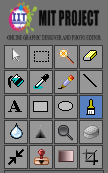
\includegraphics[width=4cm, height=5cm]{tools.png}
\caption{Toolbox.}
\end{center}
\end{figure}

\begin{figure}[h]
\begin{center}
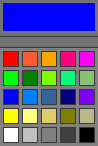
\includegraphics[width=4cm, height=5cm]{clr.png}
\caption{Color container.}
\end{center}
\end{figure}

\section{User Interface Design}
User interface (UI) design is the design of user interfaces for software or machines, such as the look of a mobile app, with a focus on ease of use and pleasurability for the user. UI design usually refers to the design of graphical user interfaces but can also refer to others, such as natural and voice user interfaces. \\

Since software is intangible, the only way a user can control or interact with it is through a designed user interface. A well designed user interface creates a user experience that the designer intended and/or a user experience that the user appreciates. \\

Design steps are as follows:

\begin{itemize}
\item \textbf{Designing the process:} Defining the subset of this process to get started.
\item \textbf{Defining strategy:} This process involves the interplay between design and business strategy.
\item \textbf{Sketching:} It provides a quick and easy way to focus and organize.
\item \textbf{Wireframing:} A wireframe is a visual representation of content layout in a design.
\item \textbf{Mockups/Visual:} The final wireframe can be converted to final Mockups or Visual.
\item \textbf{Prototypes:} A prototype is an early sample, model, or release of a product built to test a concept or process or to act as a thing to be replicated or learned from.
\end{itemize}

\section{Use Case Diagrams}
A use case diagram at its simplest is a representation of a user's interaction with the system that shows the relationship between the user and the different use cases in which the user is involved. A use case diagram can identify the different types of users of a system and the different use cases and will often be accompanied by other types of diagrams as well. \\

The use case diagram of this web application is given as follows: \\

\begin{figure}[h]
\begin{center}
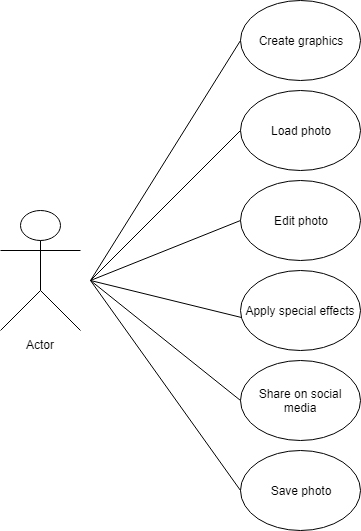
\includegraphics[width=6.5cm, height=9cm]{ucd.jpg}
\caption{Use Case Diagram.}
\end{center}
\end{figure}

\section{Responsive web design}
Responsive web design (RWD) is an approach to web design which makes web pages render well on a variety of devices and window or screen sizes. Recent work also considers the viewer proximity as part of the viewing context as an extension for RWD. Content, design and performance are necessary across all devices to ensure usability and satisfaction. \\

A site designed with RWD adapts the layout to the viewing environment by using fluid, proportion-based grids, flexible images, and CSS3 media queries, an extension of the @media rule, in the following ways:

\begin{itemize}
\item The fluid grid concept calls for page element sizing to be in relative units like percentages, rather than absolute units like pixels or points.

\item Flexible images are also sized in relative units, so as to prevent them from displaying outside their containing element.

\item Media queries allow the page to use different CSS style rules based on characteristics of the device the site is being displayed on, most commonly the width of the browser.
\end{itemize}

Responsive web design has become more important as the amount of mobile traffic now accounts for more than half of total internet traffic. Therefore, Google announced Mobilegeddon in 2015, and started to boost the ratings of sites that are mobile friendly if the search was made from a mobile device. Responsive web design is an example of user interface plasticity. \\

\textit{``Online Graphic Designer and Photo Editor"} is a responsive web application. The view of this web application on different device is shown as follows:

\begin{figure}[h]
\begin{center}
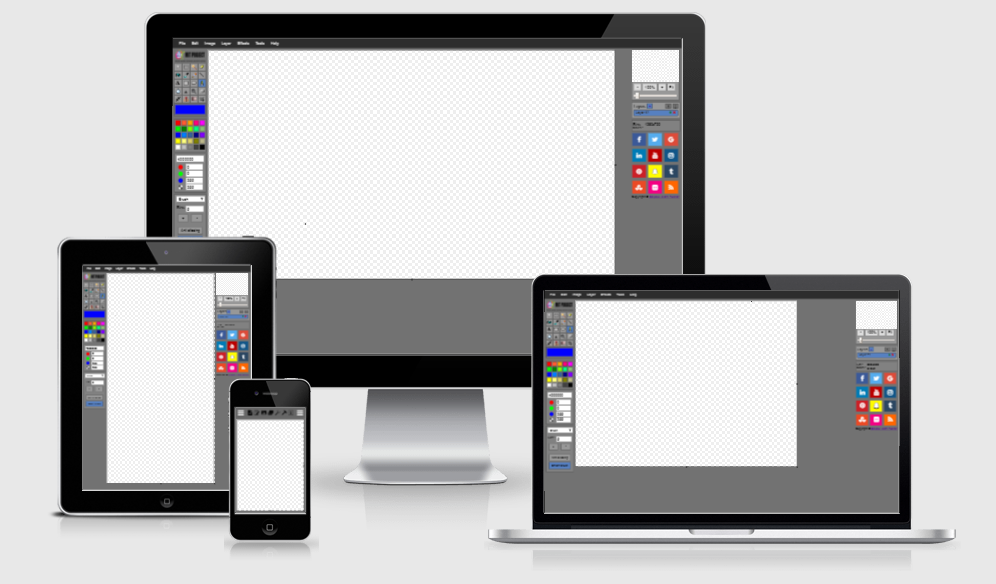
\includegraphics[width=10cm, height=7cm]{rps.png}
\caption{Responsive overview.}
\end{center}
\end{figure}

\begin{figure}[h]
\begin{center}
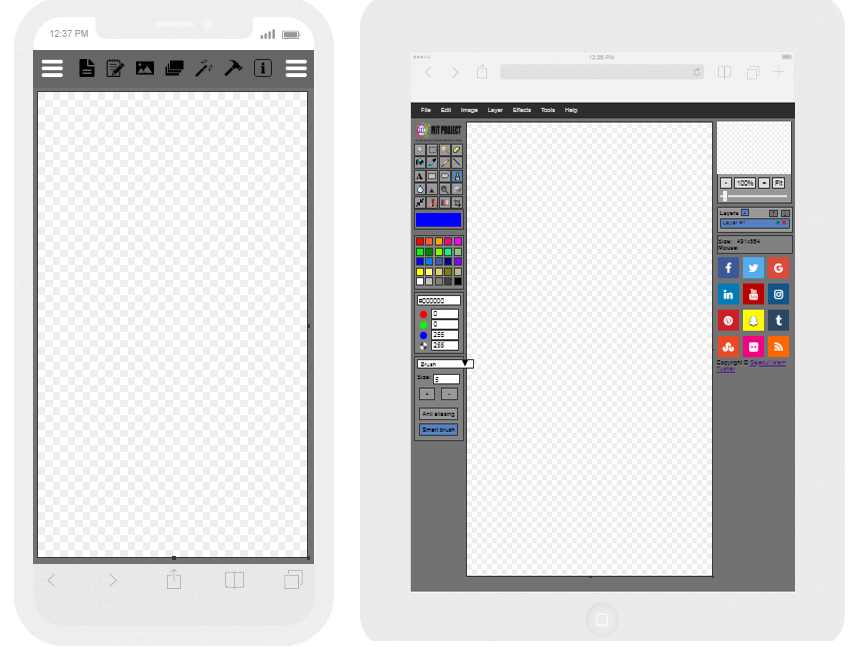
\includegraphics[width=7cm, height=5.5cm]{pot.jpg}
\caption{Portrait view.}
\end{center}
\end{figure}

\begin{figure}[h]
\begin{center}
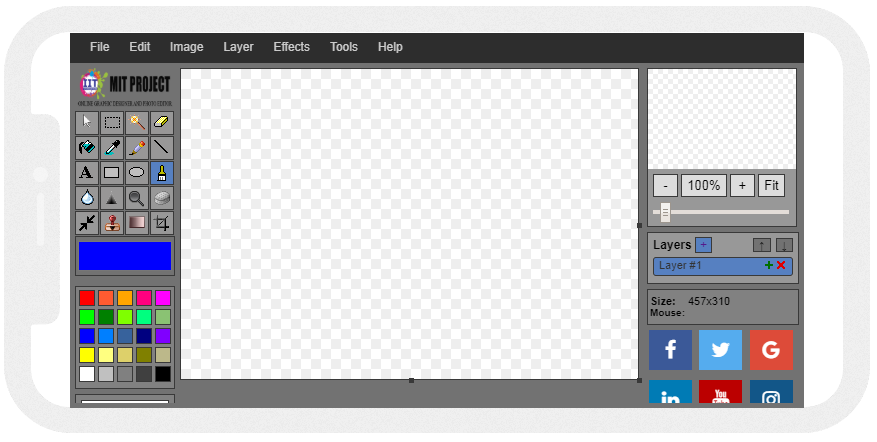
\includegraphics[width=14cm, height=7cm]{ls2.png}
\caption{Landscape view on phone.}
\end{center}
\end{figure}

\begin{figure}[h]
\begin{center}
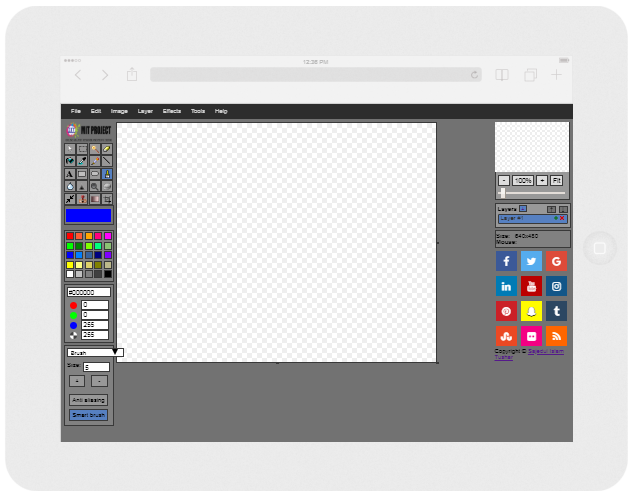
\includegraphics[width=13cm, height=10cm]{ls1.png}
\caption{Landscape view on tablet.}
\end{center}
\end{figure}


\chapter{Overview of Technologies Used}

\section{About HTML}
HTML, which stands for Hyper Text Markup Language, is the predominant markup language for web pages. It provides a means to create structured documents by denoting structural semantics for text such as headings, paragraphs, lists etc as well as for links, quotes, and other items. It allows images and objects to be embedded and can be used to create interactive forms. It is written in the form of HTML elements consisting of ``tags" surrounded by angle brackets within the web page content. It can include or can load scripts in languages such as JavaScript which affect the behavior of HTML processors like Web browsers; and Cascading Style Sheets (CSS) to define the appearance and layout of text and other material. The W3C, maintainer of both HTML and CSS standards, encourages the use of CSS over explicit presentational markup.\\

Hyper Text Markup Language(HTML) is the encoding scheme used to create and format a web document. A user need not be an expert programmer to make use of HTML for creating hypertext documents that can be put on the internet. Most graphical e-mail clients allow the use of a subset of HTML (often ill-defined) to provide formatting and semantic markup not available with plain text. This may include typographic information like coloured headings, emphasized and quoted text, inline images and diagrams. Many such clients include both a GUI editor for composing HTML e-mail messages and a rendering engine for displaying them. Use of HTML in e-mail is controversial because of compatibility issues, because it can help disguise phishing attacks, because it can confuse spam filters and because the message size is larger than plain text.\\

\noindent \textbf{Naming Conventions:}
The most common filename extension for files containing HTML is .html. A common abbreviation of this is .htm, which originated because some early operating systems and file systems, such as DOS and FAT, limited file extensions to three letters.\\

\noindent \textbf{HTML Application:}
An HTML Application is a Microsoft Windows application that uses HTML and Dynamic HTML in a browser to provide the application's graphical interface. A regular HTML file is confined to the security model of the web browser, communicating only to web servers and manipulating only webpage objects and site cookies. An HTA runs as a fully trusted application and therefore has more privileges, like creation/editing/removal of files and Windows Registry entries. Because they operate outside the browser's security model, HTAs cannot be executed via HTTP, but must be downloaded (just like an EXE file) and executed from local file system.

\section{About CSS}
Cascading Style Sheets (CSS) is a style sheet language used for describing the presentation of a document written in a markup language like HTML. CSS is a cornerstone technology of the World Wide Web, alongside HTML and JavaScript. \\

CSS is designed to enable the separation of presentation and content, including layout, colors, and fonts. This separation can improve content accessibility, provide more flexibility and control in the specification of presentation characteristics, enable multiple web pages to share formatting by specifying the relevant CSS in a separate .css file, and reduce complexity and repetition in the structural content. \\

Separation of formatting and content also makes it feasible to present the same markup page in different styles for different rendering methods, such as on-screen, in print, by voice (via speech-based browser or screen reader), and on Braille-based tactile devices. CSS also has rules for alternate formatting if the content is accessed on a mobile device. \\

The name cascading comes from the specified priority scheme to determine which style rule applies if more than one rule matches a particular element. This cascading priority scheme is predictable. \\

The CSS specifications are maintained by the World Wide Web Consortium (W3C). Internet media type (MIME type) text/css is registered for use with CSS by RFC 2318 (March 1998). The W3C operates a free CSS validation service for CSS documents. In addition to HTML, other markup languages support the use of CSS, including XHTML, plain XML, SVG, and XUL.


\section{About JavaScript}
JavaScript is an object-oriented scripting language used to enable programmatic access to objects within both the client application and other applications. It is primarily used in the form of client-side JavaScript, implemented as an integrated component of the web browser, allowing the development of enhanced user interfaces and dynamic websites. JavaScript is a dialect of the ECMAScript standard and is characterized as a dynamic, weakly typed, prototype-based 
language with first-class functions. JavaScript was influenced by many languages and was designed to look like Java, but to be easier for non-programmers to work with.\\

JavaScript uses prototypes instead of classes for inheritance. It is possible to simulate many class-based features with prototypes in JavaScript. Functions double as object constructors along with their typical role. Prefixing a function call with new creates a new object and calls that function with its local this keyword bound to that object for that invocation. The constructor's prototype property determines the object used for the new object's internal prototype. \\

JavaScript's built-in constructors, such as Array, also have prototypes that can be modified. Unlike many object-oriented languages, there is no distinction between a function definition and a method definition. Rather, the distinction occurs during function calling; a function can be called as a method. When a function is called as a method of an object, the function's local this keyword is bound to that object for that invocation.\\

The primary use of JavaScript is to write functions that are embedded in or included from HTML pages and interact with the Document Object Model (DOM) of the page. Because JavaScript code can run locally in a user's browser (rather than on a 
remote server) it can respond to user actions quickly, making an application feel more responsive. Furthermore, JavaScript code can detect user actions which HTML alone cannot, such as individual keystrokes. Applications such as Gmail take advantage of this: much of the user-interface logic is written in JavaScript, and JavaScript dispatches requests for information (such as the content of an e-mail message) to the server. The wider trend of Ajax programming similarly 
exploits this strength. \\

A JavaScript engine (also known as JavaScript interpreter or JavaScript implementation) is an interpreter that interprets JavaScript source code and executes the script accordingly. The first JavaScript engine was created by Brendan Eich at Netscape Communications Corporation, for the Netscape Navigator web browser. A web browser is by far the most common host 
environment for JavaScript. Web browsers typically use the public API to create ``host objects" responsible for reflecting the DOM into JavaScript.

\section{jQuery and JSON Introduction}

\subsection{jQuery}
jQuery is a cross-platform JavaScript library designed to simplify the client-side scripting of HTML. It is free, open-source software using the permissive MIT License. Web analysis indicates that it is the most widely deployed JavaScript library by a large margin. \\

jQuery's syntax is designed to make it easier to navigate a document, select DOM elements, create animations, handle events, and develop Ajax applications. jQuery also provides capabilities for developers to create plug-ins on top of the JavaScript library. This enables developers to create abstractions for low-level interaction and animation, advanced effects and high-level, themeable widgets. The modular approach to the jQuery library allows the creation of powerful dynamic web pages and Web applications. \\

The set of jQuery core features: DOM element selections, traversal and manipulation enabled by its selector engine (named ``Sizzle" from v1.3), created a new ``programming style", fusing algorithms and DOM data structures. This style influenced the architecture of other JavaScript frameworks like YUI v3 and Dojo, later stimulating the creation of the standard Selectors API. \\

Microsoft and Nokia bundle jQuery on their platforms. Microsoft includes it with Visual Studio for use within Microsoft's ASP.NET AJAX and ASP.NET MVC frameworks while Nokia has integrated it into the Web Run-Time widget development platform.

\subsection{JSON}

In computing, JavaScript Object Notation or JSON is an open-standard file format that uses human-readable text to transmit data objects consisting of attribute value pairs and array data types (or any other serializable value). It is a very common data format used for asynchronous browser-server communication, including as a replacement for XML in some AJAX-style systems. \\

JSON is a language-independent data format. It was derived from JavaScript, but as of 2017 many programming languages include code to generate and parse JSON-format data. The official Internet media type for JSON is application/json. JSON filenames use the extension .json. \\

Douglas Crockford originally specified the JSON format in the early 2000s; two competing standards, RFC 8259 and ECMA-404, defined it in 2017. The ECMA standard describes only the allowed syntax, whereas the RFC covers some security and interoperability considerations. \\

A restricted profile of JSON, known as I-JSON (short for ``Internet JSON"), seeks to overcome some of the interoperability problems with JSON. It is defined in RFC 7493.

\chapter{Implementation}
Implementation is the stage in the project where the theoretical design is turned into a working system and is giving 
confidence on the new system for the users that it will work efficiently and effectively. It involves careful planning, investigation of the current system and its constraints on implementation, design of methods to achieve the change over, an evaluation, of change over methods. Apart from planning major task of preparing the implementation are education and training of users. The more complex system being implemented, the more involved will be the system analysis and the design effort required just for implementation. \\

An implementation co-ordination committee based on policies of individual organization has been appointed. The implementation process begins with preparing a plan for the implementation of the system. According to this plan, the activities are to be carried out, discussions are made regarding the equipment and resources and the additional equipment has to be acquired to implement the new system. \\

It involves careful planning, investigation of the current system and its constraints on implementation, design of methods to achieve the change over and an evaluation of change over methods a part from planning. Two major tasks of preparing the implementation are education and training of the users and testing of the system. \\

The more complex the system being implemented, the more involved will be the systems analysis and design effort required just for implementation. \\
                
The implementation phase comprises of several activities. The required hardware and software acquisition is carried out. The system may require some software to be developed. For this, programs are written and tested. The user then changes over to his new fully tested system and the old system is discontinued. \\

Implementation is the final and important phase. This is the most critical stage in achieving a successful new system and in giving the users confidence that the new system will work is effective. The system can be implemented only after thorough testing. This method also offers the greatest security since the old system can take over if the errors are found or inability to handle certain type of transactions while using the new system. \\


\chapter{Testing}
The testing phase is an important part of software development. It is the puterized system will help in automate  process of finding errors and missing operations and also a complete verification to determine whether the objectives are met and the user requirements are satisfied. \\

Testing is a process of executing a program with the indent of finding an error. Testing is a crucial element of software quality assurance and presents ultimate review of specification, design and coding. System Testing is an important phase. Testing represents an interesting anomaly for the software. Thus a series of testing are performed for the proposed system before the system is ready for user acceptance testing. \\

A good test case is one that has a high probability of finding an as undiscovered error. A successful test is one that uncovers an as undiscovered error. \\

\section{Testing Objectives}
\begin{itemize} 
\item Testing is a process of executing a program with the intent of finding an error. 
\item A good test case is one that has a probability of finding an as yet undiscovered error. 
\item A successful test is one that uncovers an undiscovered error.
\end{itemize}

\section{Testing Principles}
\begin{itemize} 
\item All tests should be traceable to end user requirements.
\item Tests should be planned long before testing begins.
\item Testing should begin on a small scale and progress towards testing in large.
\item Exhaustive testing is not possible.
\item To be most effective testing should be conducted by a independent third party.
\end{itemize}

\noindent Software testing is carried out in three steps: 

\begin{itemize}   
\item The first includes unit testing, where in each module is tested to provide its correctness, validity and also determine any missing operations and to verify whether the objectives have been met. Errors are noted down and corrected immediately. Unit testing is the important and major part of the project. So errors are rectified easily in particular module and program clarity is increased. In this project entire system is divided into several modules and is developed individually.  So unit testing is conducted to individual modules. 

\item The second step includes Integration testing. It need not be the case, the software whose modules when run individually and showing perfect results, will also show perfect results when run as a whole. The individual modules are clipped under this major module and tested again and verified the results. This is due to poor interfacing, which may results in data being lost across an interface. A module can have inadvertent, adverse effect on any other or on the global data structures, causing serious problems. 

\item The final step involves validation and testing which determines which the software functions as the user expected. Here also some modifications were. In the completion of the project it is satisfied fully by the end user. 
\end{itemize}

\section{Test Cases}
 
Test cases are derived to ensure that all statements in the program have been executed at least once during testing and that all logical conditions have been executed. \\

Using White-Box testing methods, the software engineer can drive test cases that:
\begin{itemize}
\item Guarantee that logical decisions on their true and false sides. 
\item Exercise all logical decisions on their true and false sides.  
\item Execute all loops at their boundaries and with in their operational bounds.  
\item Exercise internal data structure to assure their validity. 
\end{itemize}
The test case specification for system testing has to be submitted for review before system testing commences.

\chapter{Operation and Maintenance}
As the number of computer based systems, grieve libraries of computer software began to expand. In house developed projects produced tones of thousand soft program source statements. Software products purchased from the outside added hundreds of thousands of new statements. A dark cloud appeared on the horizon. All of these programs, all of those source statements-had to be corrected when false were detected, modified as user requirements changed, or adapted to new hardware that was purchased. These activities were collectively called software Maintenance. \\

The maintenance phase focuses on change that is associated with error correction, adaptations required as the software's environment evolves, and changes due to enhancements brought about by changing customer requirements. Four types of changes are encountered during the maintenance phase: 

\begin{itemize}
\item Correction.
\item Adaptation.
\item Enhancement. 
\item Prevention.
\end{itemize}

\section{Correction}
Even with the best quality assurance activities is lightly that the customer will uncover defects in the software. Corrective maintenance changes the software to correct defects. \\
 
Maintenance is a set of software Engineering activities that occur after software has been delivered to the customer and put into operation. Software configuration management is a set of tracking and control activities that began when a software project begins and terminates only when the software is taken out of the operation. \\
 
We may define maintenance by describing four activities that are undertaken after a program is released for use: 
\begin{itemize}
\item Corrective Maintenance 
\item Adaptive Maintenance 
\item Perfective Maintenance or Enhancement 
\item Preventive Maintenance or re-engineering 
\end{itemize}  
           
Only about 20 percent of all maintenance work are spent ``fixing mistakes". The remaining 80 percent are spent adapting existing systems to changes in their external environment, making enhancements requested by users, and re-engineering an application for use. \\

\section{Adaptation} 
Over time, the original environment (e.g: CPU, operating system, business rules, external product characteristics) for which the software was developed is likely to change. Adaptive maintenance results in modification to the software to accommodate change to its external environment.
 
\section{Enhancement}
As software is used, the customer/user will recognize additional functions that will provide benefit. Perceptive maintenance extends the software beyond its original function requirements. 

\section{Prevention}
Computer software deteriorates due to change, and because of this, preventive maintenance, often called software re engineering, must be conducted to enable the software to serve the needs of its end users. In essence, preventive maintenance makes changes to computer programs so that they can be more easily corrected, adapted, and enhanced.  Software 
configuration management (SCM) is an umbrella activity that is applied throughout the software process. \\

However, considering all the discussion above the operation and maintenance of this web application is very easy. The major emphasis is given to the development and integration of this web application.

\chapter{Conclusion and Scope for Further Development}
The system has been developed and tested with proper care. The system results in regular timing preparation of the required output. In  comparison with the manual system, this system is able to save the time, cost and effort of the work. \\

\textit{``Online Graphic Designer and Photo Editor"} is designed in such a way that future modifications can be done easily. For the further development of this project such as providing pro-services only to the registered users and business or commercial project implementation the requirements are: 

\begin{itemize}
\item \textbf{Web Language:} PHP 
\item  \textbf{Web Server:} Apache or Wamp Server 
\item  \textbf{Database:} MySQL
\end{itemize}

The further development of this application will not be so difficult and this will enable some new features and security like authentication, authorization and availability of the premium features to this web application. \\

However, The following conclusions can be deduced from the development of the project.

\begin{itemize}
\item The system is reliable.
\item It provides a friendly graphical user interface which proves to be better when compared to the existing system.   
\item System security, data security and reliability are the striking features. 
\item The System has adequate scope for modification in future if it is necessary. 
\end{itemize}

\noindent \textit{``Online Graphic Designer and Photo Editor"} is very user friendly and helpful for the designers and editors. By using this web application they can easily perform their designing or editing tasks in a better and efficient way. It will also save their time, cost and effort of the work.

\begin{thebibliography}{widestlabel}


\bibitem{CSS} Cascading Style Sheets. \emph{https://en.wikipedia.org/wiki/Cascading\_Style\_Sheets}\hspace{.07cm}.

\bibitem{Dreamtech} Dreamtech, W.  \emph{HTML 5.0 Black Book} Dreamtech Press.

\bibitem{Elias} Elias, M. Awad \emph{Systems Analysis and Design} Galgotia Publications Pvt. Ltd.

\bibitem{Jacobson} Jacobson, R. and Wurman, R.S.  \emph{Information Design (MIT Press)}

\bibitem{jQuery} jQuery. \emph{https://en.wikipedia.org/wiki/JQuery}\hspace{.07cm}.

\bibitem{JSON} JSON. \emph{https://en.wikipedia.org/wiki/JSON}\hspace{.07cm}.

\bibitem{Robbins} Robbins, J.M. \emph{Learning Web Design (4th Edition)} (John Wiley \& Sons Inc.)

\bibitem{ViliusL} viliusle, \emph{miniPaint} (https://github.com/viliusle/miniPaint).

\bibitem{Welling} Welling, L. and Thomson, L.  \emph{PHP and MySQL Web Development (4th Edition).}

\bibitem{W3Schools} W3Schools CSS Tutorial \emph{https://www.w3schools.com/css/}

\bibitem{W3Schools} W3Schools jquery Tutorial \emph{https://www.w3schools.com/jquery/default.asp}


\end{thebibliography}

\end{document}